\subsection{SP-26 (PST)}
Pravidla pro výpočty pravděpodobností, Bayesův vzorec. Náhodné veličiny, příklady rozdělení, distribuční funkce, hustota, momenty. Nezávislost náhodných jevů a veličin. Centrální limitní věta, zákony velkých čísel.

\subsubsection*{Náhodný experiment}
\begin{itemize}
	\item je reprezentován pravděpodobnostním prostorem $(\Omega, \mathcal{F}, P)$
	\item $\Omega$ je množina možných výsledků (elementárních jevů)
	\begin{itemize}
		\item vzájemně exklusivní --- mělo by být vždy jednoznačné, který elementární jev nastal
		\item v souhrnu vyčerpávající --- vše co se může stát je popsáno elementárními jevy
	\end{itemize}
	\item $\mathcal{F}$ je systém podmnožin $\Omega$ s rozumnými vlastnostmi ($\sigma$-algebra)
	\begin{itemize}
		\item $\mathcal{F}$ obsahuje nemožný jev
		\item pokud $A \in \mathcal{F}$, tak $\mathcal{F}$ obsahuje i opačný jev (značeno $A^c$ jako doplněk)
		\item obsahuje spočetné sjednocení jevů
	\end{itemize}
	\item prvky $A \in \mathcal{F}$ jsou náhodné jevy
	\item pravděpodobnostní míra $P$ je funkce, která přiřazuje náhodným jevům reálné číslo z intervalu $\langle 0,1 \rangle$, reprezentující ideální podíl případů, kdy jev nastává 
\end{itemize}

\subsubsection*{Podmíněná pravděpodobnost}
Pravděpodobnost jevu za předpokladu, že nastal jiný jev. $$P(A|B) = \frac{P(A \cap B)}{P(B)}$$

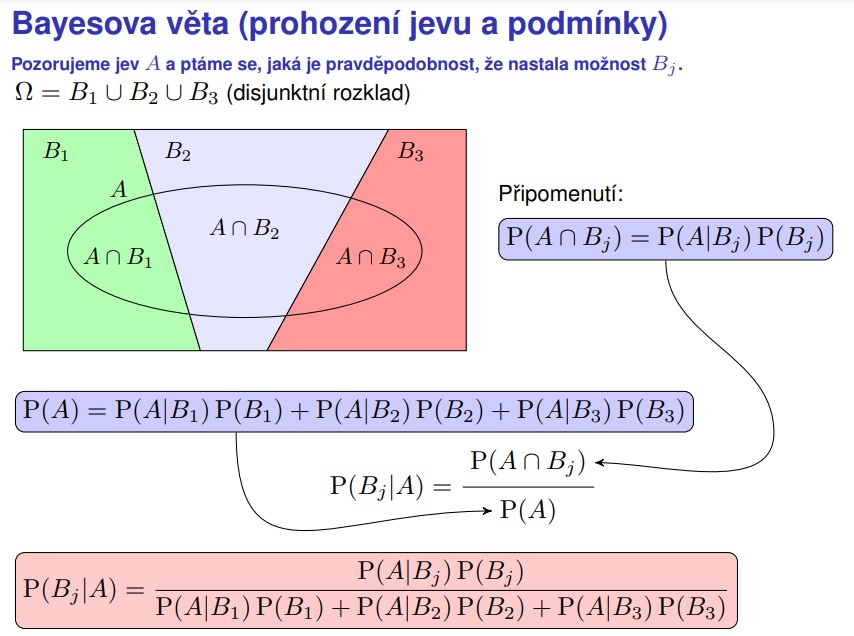
\includegraphics[width=0.8\textwidth]{img/SP-26_0.jpg}

\subsubsection*{Nezávislé jevy}
\begin{itemize}
	\item Jevy A a B jsou nezávislé, pokud $P(A \cap B) = P(A) \cdot P(B)$.
	\item Nezávislé jevy se neovlivňují --- $P(A|B) = P(A), \quad P(B|A) = P(B)$
\end{itemize}

\subsubsection*{Náhodné veličiny}
Pro matematické zpracování se každému výsledku $\omega \in \Omega$ přiřadí číslo. Přiřazení čísla vybíráme dle potřeby, podle toho co zrovna zkoumáme.
\begin{itemize}
	\item Náhodná veličina $X$ na pravděpodobnostním prostoru $(\Omega, \mathcal{F}, P)$ je funkce, která každému výsledku experimentu $\omega  \in \Omega$  přiřadí hodnotu $X(\omega) \in \mathbb{R}$ a pro kterou platí podmínka měřitelnosti $\{X \leq x\} \in \mathcal{F}, \forall x \in \mathbb{R}$.
	\item Distribuční funkce náhodné veličiny $X$ je definovaná vztahem $F_X(x) = P(X \leq x)$.
	\item Diskrétní náhodné veličiny mají pravděpodobnostní funkci, spojité hustotu (vždy derivace distribuční funkce).
\end{itemize}

\subsubsection*{Střední hodnota}
\begin{itemize}
	\item střední hodnota diskrétních veličin: $$\text{E}X = \sum_k x_k P(X = x_k)$$
	\item střední hodnota spojitých veličin: $$\text{E}X = \int_{-\infty}^{+\infty} xf(x)\text{d}x$$
\end{itemize}

\subsubsection*{Rozptyl}
\begin{itemize}
	\item Rozptyl (variance): $$\text{var}X = \text{E}[(X-\text{E}X)^2]$$
	\item nejlépe se vypočítá jako $\text{var}X = \text{E}X^2 - (\text{E}X)^2$
	\item směrodatná odchylka: $$\text{sd}X = \sqrt{\text{var}X}$$
\end{itemize}

\subsubsection*{Momenty}
Pro $k \in \mathbb{N}$ definujeme:
\begin{itemize}
	\item $k$-tý moment náhodné veličiny $X$:
	
	$$\mu_k = \text{E}(X^k) = \sum_{\text{all }x_i} x_i^k P(X = x_i) \text{ pro } X \text{ diskrétní}$$
	$$\mu_k = \text{E}(X^k) = \int_{-\infty}^{+\infty} x^k f_X(x)\text{d}x \text{ pro } X \text{ diskrétní}$$
	\item $k$-tý centrální moment veličiny $X$:
	$$\sigma_k = \text{E}(X-\text{E}X)^k = \sum_{\text{all }x_i} (x_i - \mu_1)^k P(X = x_i) \text{ pro } X \text{ diskrétní}$$
	$$\sigma_k = \text{E}(X-\text{E}X)^k = \int_{-\infty}^{+\infty} (x - \mu_1)^k f_X(x)\text{d}x \text{ pro } X \text{ diskrétní}$$
\end{itemize}

\subsubsection*{Diskrétní rozdělení}
\begin{itemize}
	\item Bernoulliho (Alternativní) rozdělení
	
	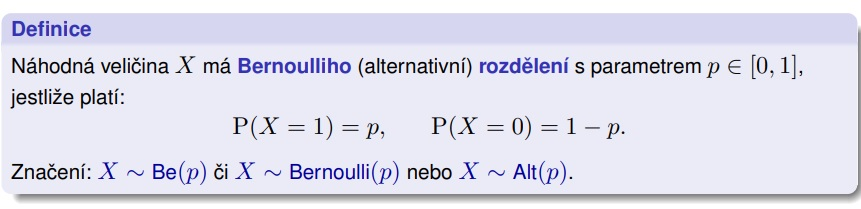
\includegraphics[width=0.7\textwidth]{img/SP-26_1.jpg}
	
	\begin{itemize}
		\item $\text{E}X = p$
		\item $\text{var}X = p(1-p)$
	\end{itemize}
	
	\item Binomické rozdělení --- opakované hody, zajímá nás pravděpodobnost že právě $n$-krát padne např. hlava --- výpočet $P(\text{X} = k) = \binom{n}{k} p^k (1-p)^{n-k}$
	\begin{itemize}
		\item $\text{E}X = np$
		\item $\text{var}X = np(1-p)$
	\end{itemize}
	
	\item Geometrické rozdělení --- opakované hody, zajímá nás pravděpodobnost že právě na $k$-tý pokus padne poprvé např. hlava --- výpočet $P(\text{X} = k) = (1-p)^{k-1} p$
	\begin{itemize}
		\item $\text{E}X = \frac{1}{p}$
		\item $\text{var}X = \frac{1-p}{p^2}$
	\end{itemize}
	
	\item Poissonovo rozdělení --- zajímá nás např počet jevů za určitý čas, je to aproximace, limita binomického do nekonečna
	
\end{itemize}

\subsubsection*{Spojitá rozdělení}
\begin{itemize}
	\item rovnoměrné rozdělení
	\item exponenciální rozdělení
	\item normální rozdělení
\end{itemize}

\subsubsection*{Nezávislost náhodných veličin}
Náhodné veličiny $X$ a $Y$ nazýváme nezávislé, pokud pro všechna $x, y \in \mathbb{R}$ jsou jevy $\{X \leq x\}$ a $\{Y \leq y\}$ nezávislé. Tedy pokud platí: $$P(X \leq x \cap Y \leq y) = P(X\leq x) \cdot P(Y \leq y) $$
Lze také vyjádřit pomocí hustot/pravděpodobnostních funkcí:
$$P(X = x \cap Y = y) = P(X = x) \cdot P(Y = y) $$

\subsubsection*{Limitní věty}
Místo samotných náhodných veličin řešíme jejich posloupnosti, které vznikly opakováním experimentu. Co nás typicky zajímá:
\begin{itemize}
	\item průměr (aritmetický): $$\bar{X}_n = \frac{1}{n}\sum_{i = 1}^n X_i$$
	\item součet: $$S_n = \sum_{i = 1}^n X_i $$
\end{itemize}
kde $X_1,...,X_n$ jsou nezávislé náhodné veličiny se stejným rozdělením (I.I.D.).

\subsubsection*{Zákony velkých čísel}
\begin{itemize}
	\item Slabý zákon velkých čísel: $X_1,...,X_n$ jsou i.i.d. s konečnou střední hodnotou $\text{E}X_i = \mu$ a konečným rozptylem $\sigma^2$. Potom $ \bar{X}_n$ konverguje k $\mu$ v pravděpodobnosti: $$\bar{X}_n \xrightarrow{P} \mu \quad \text{ pro } \quad n\to\infty $$
	Jinak řečeno, pro $n\to\infty$ je pravděpodobnost nenulové vzdálenosti průměru od $\mu$ nulová.
	
	\item Silný zákon velkých čísel: $X_1,...,X_n$ jsou i.i.d. se střední hodnotou $\text{E}X_i = \mu$ . Potom $\bar{X}_n$ konverguje k $\mu$ skoro jistě (s pravděpodobností 1).
\end{itemize}

\subsubsection*{CLV --- Centrální limitní věta}
Nechť $X_1,X_2,...$ je posloupnost i.i.d. náhodných veličin s konečnou střední hodnotou $\text{E}X_i = \mu$ a konečným rozptylem $\text{var}X_i = \sigma^2 > 0$. Potom $$\frac{\bar{X}_n - \mu}{\sigma / \sqrt{n}} \xrightarrow{\mathcal{D}} N(0,1) \quad \text{ pro } \quad n\to\infty$$
Podobně
$$\frac{S_n - n\mu}{\sigma \sqrt{n}} \xrightarrow{\mathcal{D}} N(0,1) \quad \text{ pro } \quad n\to\infty$$